\section{設計と実験}
  今回の課題は,設計と実験を実験のフィードバックをもとに繰り返して行う.
  最終的に提出する梁は,一番たわみの小さかったものとする.
  \subsection{①}
    解析条件2より梁の長さと体積が決まっている.
    そこでまずはなるべく$z$軸方向に長く条件の範囲内に収まる梁を作成する.\\\indent
    梁の接地面の横の長さをy,
    縦の長さを$z$とすると解析条件2より面積は以下のように表される.
    \begin{eqnarray}
      && y \cdot z \cdot 200 = 50000 \notag \\
      &\iff& y \cdot z = 250[mm^2] \label{eq:area}
    \end{eqnarray}
    
    ここで解析条件2より$y$は以下のように表される.
    \begin{eqnarray}
      && y^2 + z^2 = 10000 \notag \\
      &\iff& y^2 = 10000 - z^2 \notag \\
      &\iff& y = \pm \sqrt{10000-z^2} \notag \\
      &\therefore& y = \sqrt{10000-z^2} \label{eq:length_y}
    \end{eqnarray}

    よって\eqref{eq:area}より接地面の面積は以下のように変形できる,
    \begin{equation*}
      z \cdot \sqrt{10000-z^2} = 250
    \end{equation*}

    これを解く.
    \begin{eqnarray*}
      &&z  \approx 2.5008, 99.969 \\
      &\therefore &z = 99.969
    \end{eqnarray*}

    $z = 99.969$のとき\eqref{eq:length_y}より$y$の長さを求めると.\\\indent
    \begin{eqnarray*}
      && y = \sqrt{10000-99.969^2} \\
      &\therefore& y = 2.489
    \end{eqnarray*}
    
    以上より$z = 99.969,y = 2.489,L = 200$の板を梁と見立てて実験を行う.
    このときの解析条件は以下.
    \begin{gather*}
      d = \sqrt{99.96^2 + 2.82^2} = 99.99998[mm] \\
      V \approx 49765[mm^3]
    \end{gather*}

    \begin{figure}[H]
      \begin{tabular}{ccc}
        \begin{minipage}{.33\textwidth}
          \centering
          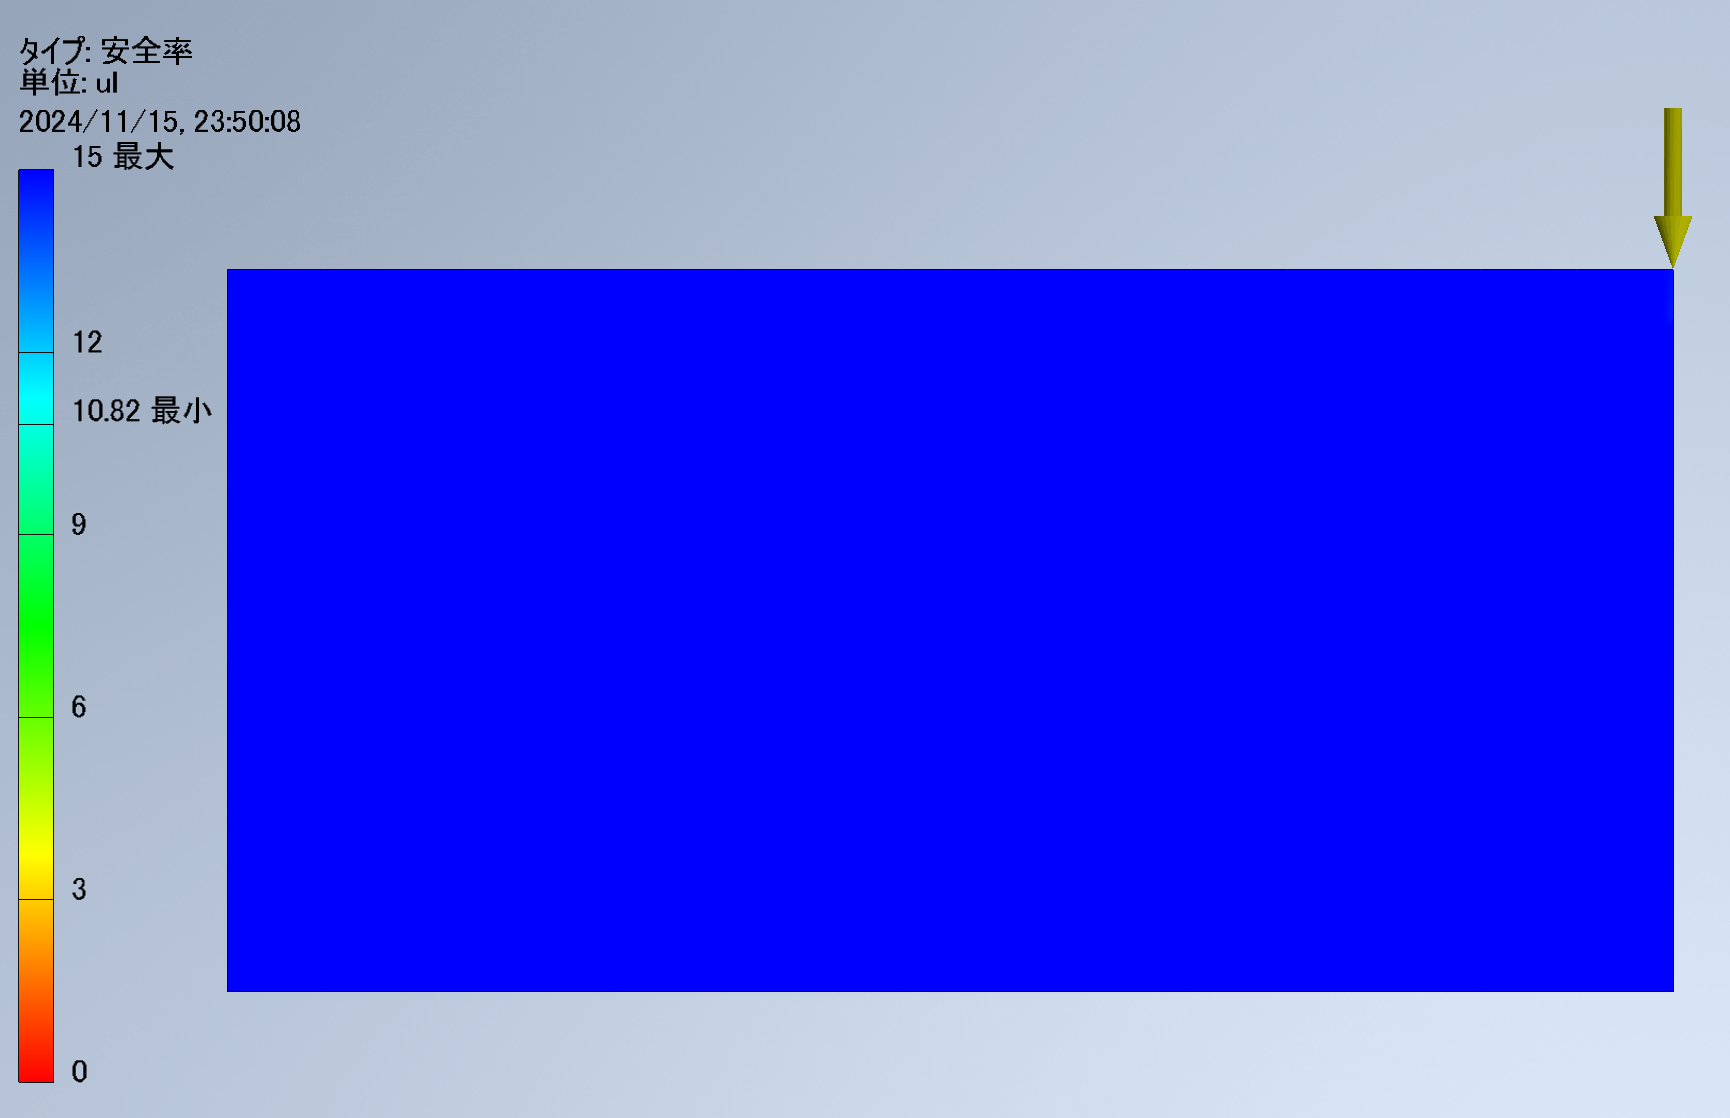
\includegraphics[width=0.99\linewidth]{images/model_1/safe.png}
          \caption{安全率}
          \label{img:safe1}
        \end{minipage}
        \begin{minipage}{.33\textwidth}
          \centering
          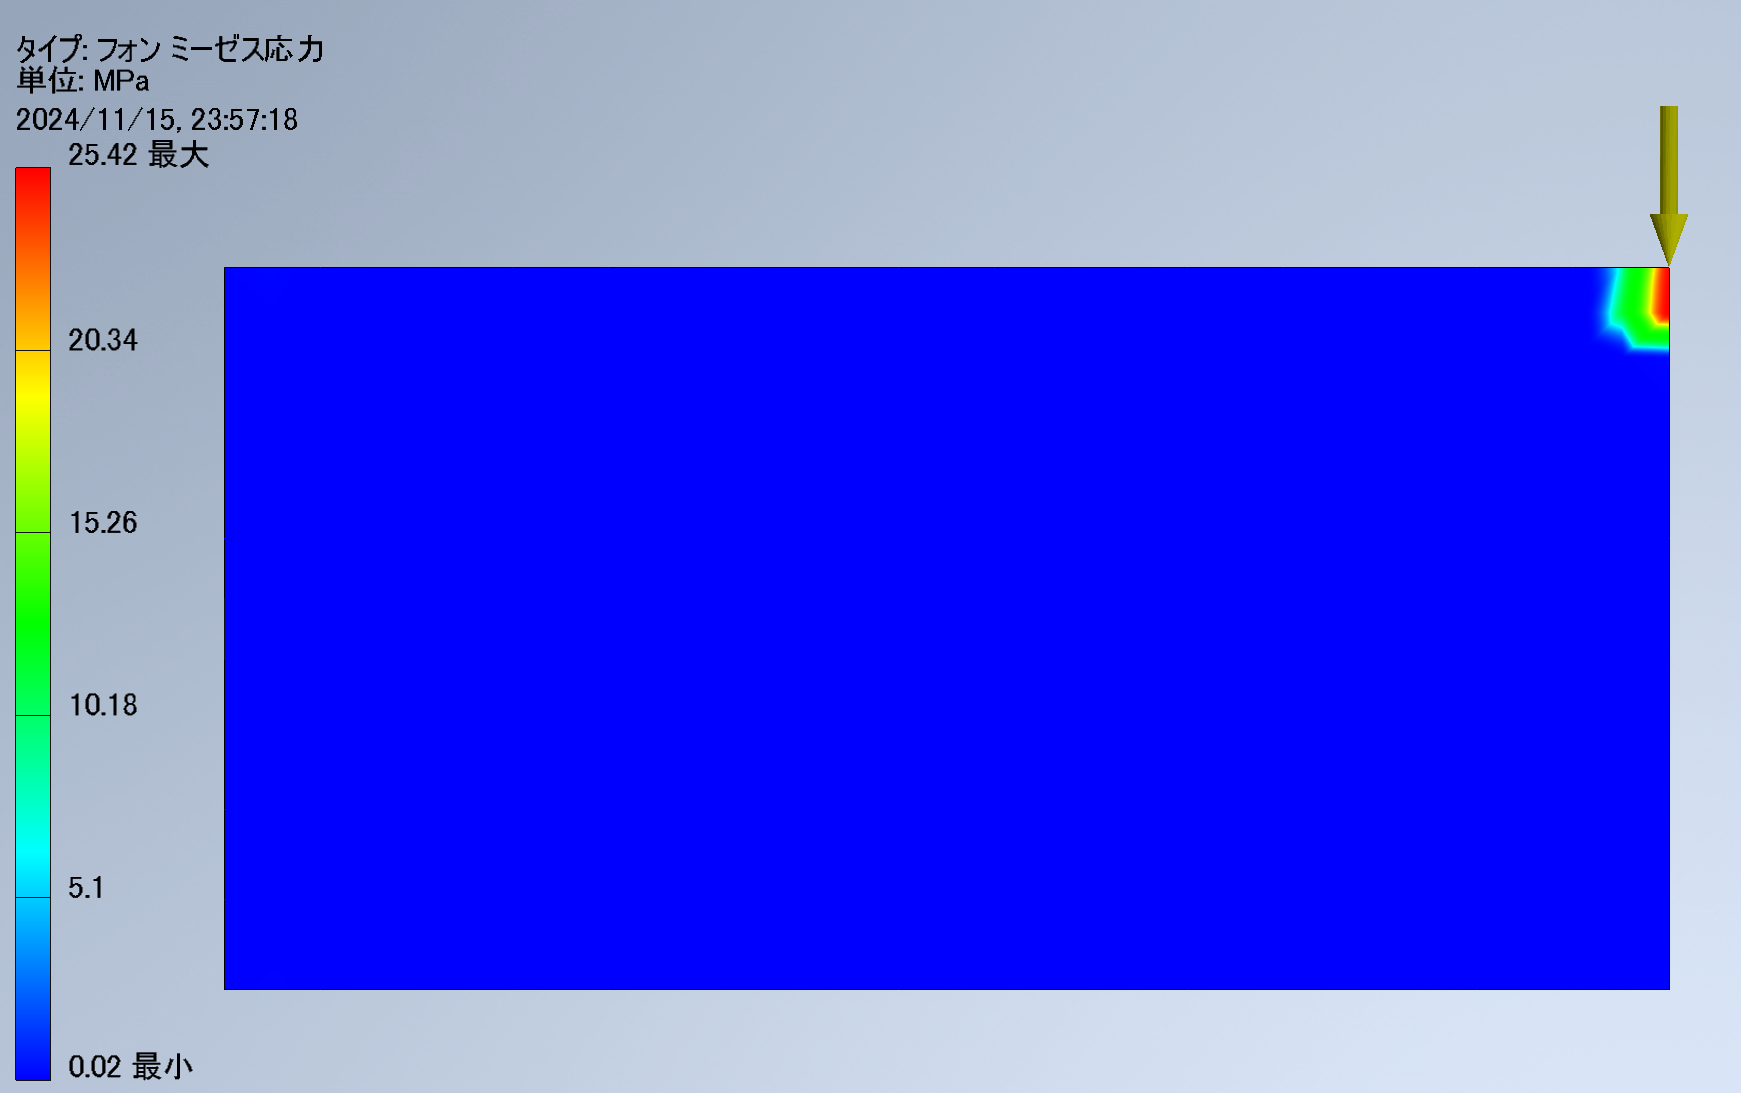
\includegraphics[width=0.99\linewidth]{images/model_1/voms.png}
          \caption{応力}
          \label{img:voms1}
        \end{minipage}
        \begin{minipage}{.33\textwidth}
          \centering
          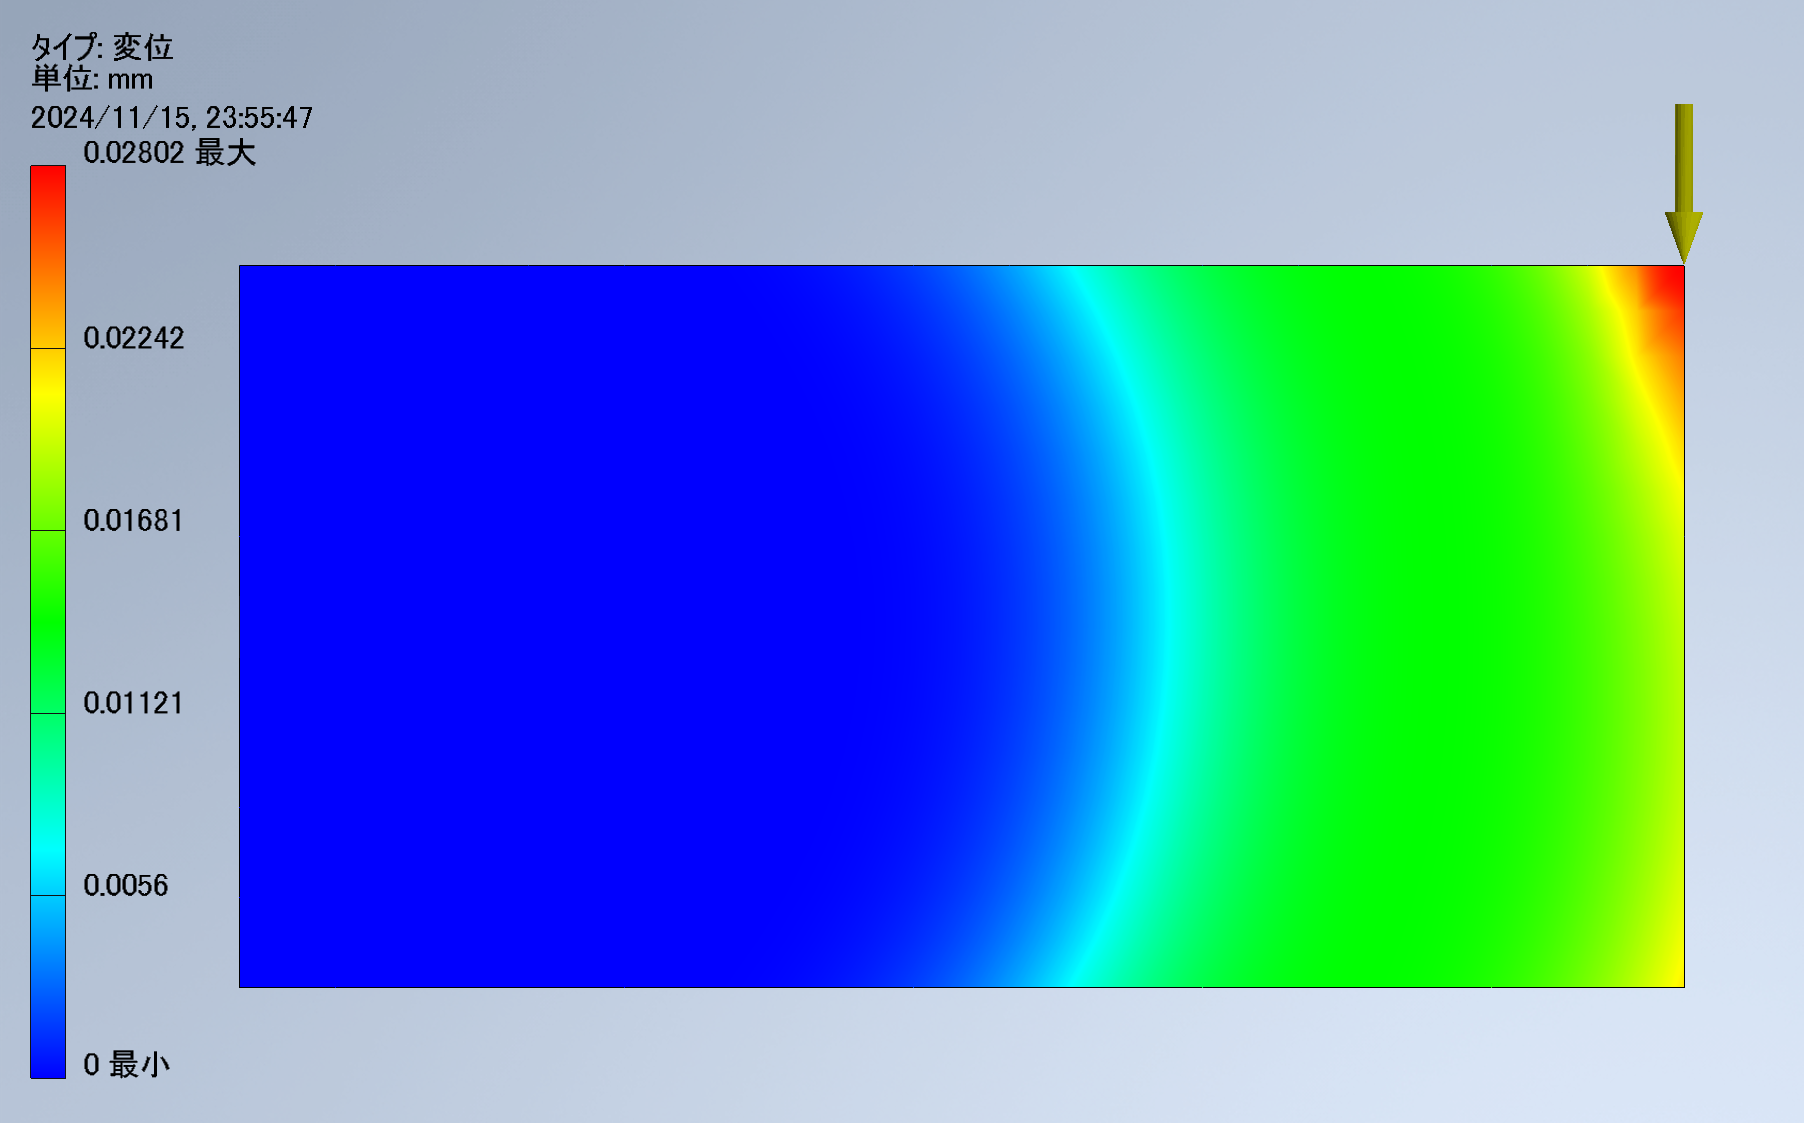
\includegraphics[width=0.99\linewidth]{images/model_1/disp.png}
          \caption{変位}
          \label{img:disp1}
        \end{minipage}
      \end{tabular}
    \end{figure}

    図1より安全率は4以上を達成している.
    図2より応力は力がかかっている付近の一部のみが強い.
    図3より変位は画像の水平左右のx軸右方向にいくに連れ大きくなっている.
    また変位は同心円状に大きくなっている.\\\indent
    次の実験は変位が大きく変化していない部分を削って行う.
    図3の青い部分には応力も安全率も安定しているため,
    大幅に梁を削ることが可能である.
